%%%%%%%% ICML 2018 EXAMPLE LATEX SUBMISSION FILE %%%%%%%%%%%%%%%%%

\documentclass{article}

% Recommended, but optional, packages for figures and better typesetting:
\usepackage{microtype}
\usepackage{graphicx}
\usepackage{subfigure}
%\usepackage{subfloat}
\usepackage{booktabs} % for professional tables

% hyperref makes hyperlinks in the resulting PDF.
% If your build breaks (sometimes temporarily if a hyperlink spans a page)
% please comment out the following usepackage line and replace
% \usepackage{icml2018} with \usepackage[nohyperref]{icml2018} above.
\usepackage{hyperref}

% Attempt to make hyperref and algorithmic work together better:
\newcommand{\theHalgorithm}{\arabic{algorithm}}

% Use the following line for the initial blind version submitted for review:
\usepackage{icml2018}

\usepackage{url}
\usepackage{color}
%\usepackage{times}
\usepackage{amsfonts}
\usepackage{amsmath}
\usepackage{amsthm}

%\usepackage{algorithm}
%\usepackage{algorithm2e}
\usepackage{indentfirst}
\usepackage{caption}
\usepackage{bm}
%\usepackage{subcaption}
\usepackage{graphicx,epsfig,latexsym,subfig}
%\usepackage{slashbox}
\usepackage{graphicx,dblfloatfix}
\numberwithin{equation}{section}
% laks macros 
\newcommand{\laks}[1]{\textcolor{black}{#1}}
\newcommand{\R}{\mathbb{R}}
\newcommand{\supX}{\sup_{X \in \mathcal{X}}}
\newcommand{\E}{\mathbb{E}}
\newtheorem{theorem}{Theorem}
\newtheorem{lemma}{Lemma}
\newtheorem{assumption}{Assumption}
\newtheorem{corollary}{Corollary}
\newtheorem{sampling strategy}{Sampling Strategy}


% If accepted, instead use the following line for the camera-ready submission:
%\usepackage[accepted]{icml2018}

% The \icmltitle you define below is probably too long as a header.
% Therefore, a short form for the running title is supplied here:
\icmltitlerunning{Submission and Formatting Instructions for ICML 2018}

\begin{document}

\twocolumn[
%\icmltitle{Large-Scale Implicit Preference Completion}
\icmltitle{Supplemetary Materials:\\ 
%Preference Completion for Large-Scale Implicit Feedback Data
}

% It is OKAY to include author information, even for blind
% submissions: the style file will automatically remove it for you
% unless you've provided the [accepted] option to the icml2018
% package.

% List of affiliations: The first argument should be a (short)
% identifier you will use later to specify author affiliations
% Academic affiliations should list Department, University, City, Region, Country
% Industry affiliations should list Company, City, Region, Country

% You can specify symbols, otherwise they are numbered in order.
% Ideally, you should not use this facility. Affiliations will be numbered
% in order of appearance and this is the preferred way.
\icmlsetsymbol{equal}{*}

\begin{icmlauthorlist}
\icmlauthor{Huang Fang}{ubc}
\icmlauthor{Liran Li}{ubc}
\icmlauthor{Michael p. Friedlander}{ubc}
\icmlauthor{Laks V.S. Lakshmanan}{ubc}
\icmlauthor{Cho-Jui Hsieh}{ucd}
\end{icmlauthorlist}

% \icmlaffiliation{to}{University of Torontoland, Torontoland, Canada}
% \icmlaffiliation{goo}{Googol ShallowMind, New London, Michigan, USA}
% \icmlaffiliation{ed}{University of Edenborrow, Edenborrow, United Kingdom}
\icmlaffiliation{ubc}{University of British Columbia, British Columbia, Canada}
\icmlaffiliation{ucd}{University of California, Davis, USA}


\icmlcorrespondingauthor{Huang Fang}{hgfang@cs.ubc.ca}
%\icmlcorrespondingauthor{Liran Li}{liran.li@cs.ubc.ca}

% You may provide any keywords that you
% find helpful for describing your paper; these are used to populate
% the "keywords" metadata in the PDF but will not be shown in the document
\icmlkeywords{Machine Learning, ICML}

\vskip 0.3in
]

% this must go after the closing bracket ] following \twocolumn[ ...

% This command actually creates the footnote in the first column
% listing the affiliations and the copyright notice.
% The command takes one argument, which is text to display at the start of the footnote.
% The \icmlEqualContribution command is standard text for equal contribution.
% Remove it (just {}) if you do not need this facility.

\printAffiliationsAndNotice{}  % leave blank if no need to mention equal contribution
%\printAffiliationsAndNotice{\icmlEqualContribution} % otherwise use the standard text.


\section{The relationship between $Y_{ijk}$ and $A_{ijk}$}

Given $Y_{ijk} = (1,1)$

\begin{equation}
\begin{aligned}
    & Pr[A_{ijk} = (1,1) ~|~ Y_{ijk} = (1,1)] = p_i^2 \\ 
    & Pr[A_{ijk} = (1,0) ~|~ Y_{ijk} = (1,1)] = p_i(1-p_i) \\
    & Pr[A_{ijk} = (0,1) ~|~ Y_{ijk} = (1,1)] = p_i(1-p_i) \\
    & Pr[A_{ijk} = (0,0) ~|~ Y_{ijk} = (1,1)] = (1-p_i)^2 \nonumber
\end{aligned}
\end{equation}
Given $Y_{ijk} = (1,0)$
\begin{equation}
\begin{aligned}
    & Pr[A_{ijk} = (1,0) ~|~ Y_{ijk} = (1,0)] = p_i \\ 
    & Pr[A_{ijk} = (0,0) ~|~ Y_{ijk} = (1,0)] = 1-p_i \\
 \nonumber
\end{aligned}
\end{equation}
Given $Y_{ijk} = (0,1)$
\begin{equation}
\begin{aligned}
    & Pr[A_{ijk} = (0,1) ~|~ Y_{ijk} = (0,1)] = p_i \\ 
    & Pr[A_{ijk} = (0,0) ~|~ Y_{ijk} = (0,1)] = 1-p_i \\
 \nonumber
\end{aligned}
\end{equation}
Given $Y_{ijk} = (0,0)$
\begin{equation}
\begin{aligned}
    & Pr[A_{ijk} = (0,0) ~|~ Y_{ijk} = (0,0)] = 1 \\ 
 \nonumber
\end{aligned}
\end{equation}

%\section{Proof for Theorem \ref{thm:noisy}}
\section{Proof of Theorem 1}


Let $$L(X) := \frac{1}{|\Omega_S|} \sum_{(i,j,k) \in \Omega_S}  \mathcal{L}( (R_{i,j} - R_{i,k})(X_{i,j} - X_{i,k}) )$$
% $\Xi$ as all possible subsets $\{ \Omega ~|~ |\Omega| = m \}$

First, it is easy to see that under uniform sampling, we have $\mathbb{E}[L(X)] = R_A(X)$. 

Then we need to bound $\sup_{X \in \mathcal{X} } |L(X) - R_A(X)| $.

\begin{lemma}
\label{lemma:bound}
    With probability at least $1 - \delta/2$, 
    \begin{equation}
    \begin{aligned}
        \supX |L(X) - R_A(X)| \leq & 2 \alpha \sqrt{\frac{2\ln(2/\delta)}{m}} + 2\alpha \sqrt{ \frac{2\ln(4/\delta) }{d_1 d_2} } \\
        & + 2 C \sqrt{\frac{(d_1 + d_2)}{m}} \ln(d_1 d_2)
    \end{aligned}
    \end{equation}
\end{lemma}

\emph{Proof:}
Break the objective into 2 parts: 
%\begin{equation}
    \begin{align}
        \supX \Big|L(X) - R_A(X)\Big| \leq \supX \Big|L(X) - \mathbb{E}_{\Omega_S} [L(X) | R] \Big| \label{eq:part1}  \\ 
        + \supX \Big|\mathbb{E}_{\Omega_S} [L(X) | R] - R_A(X) \Big| \label{eq:part2}
    \end{align}
%\end{equation}

For the first part Eq \ref{eq:part1}, it can be easily bounded by \laks{the law of large numbers, and by using Hoeffding's Inequality}.

Since $\mathcal{L}$ is 1-Lipschitz and $\underset{i,j}{\max} |X_{i,j}| \leq \alpha$, we have 
$$\Big|\mathcal{L}((R_{i,j} - R_{i,k})(X_{i,j} - X_{i,k})) - \mathcal{L}(0) \Big| \leq 2\alpha$$ 
for $\forall 1 \leq i \leq d_1, 1 \leq j \leq d_2,  X \in \mathcal{X}$.

By Applying Hoeffding's Inequality, we know that

\begin{align}
    Pr\Big\{ \big|L(X) - \E_{\Omega_S}[ L(X) | R ]  \big| \Big\} \geq \epsilon ] \leq 2 \exp\Big\{-\frac{2m \epsilon^2}{(4\alpha)^2} \Big\} \nonumber
\end{align}

Let $2 \exp\Big\{-\frac{2m \epsilon^2}{(4\alpha)^2} \Big\} = \delta/4$, then with probability at least $1 - \delta/4$,

\begin{equation}
    \begin{aligned}
        \supX |L(X) - \mathbb{E}_{\Omega_S} [L(X) | R] | \leq 2 \alpha \sqrt{\frac{2\ln(8/\delta)}{m}}
        \label{eq:res_part1}
    \end{aligned}
\end{equation}

For the second part Eq \ref{eq:part2}, $\supX \big|\mathbb{E}_{\Omega_S} [L(X) | R] - R_A(X) \big|$ is a function of $R$, since $R_{i,j} \in \{0, 1\}$ are independent from each other, we can apply McDiarmid's Inequality \cite{Mc}.

First, it is easy to show that under uniform sampling, the expected number of pairs related with $R_{i,j}$ is $\frac{2m}{d_1 d_2}$, \laks{a single change of $R_{i,j}$ would  change $\E_{\Omega_S}[L(X)|R] $ by at most $c_{ij} = \frac{1}{m} \frac{2m}{d_1 d_2} 2\alpha = \frac{4 \alpha }{d_1 d_2} $.} 

By McDiarmid's inequality, With probability at least $1 - \delta/4$,

\begin{equation}
    \begin{aligned}
    & \sup_{X \in \mathcal{X}} \big| \mathbb{E}_{\Omega_S} [L(X) | R] - R_A(X) \big| \\
    \leq & \mathbb{E}_R \Big[ \sup_{X \in \mathcal{X}} \big|\mathbb{E}_{\Omega_S} [L(X) | R] - R_A(X) \big| \Big] \\
    & + \sqrt{ \frac{\ln(4/\delta) \sum c_{ij}^2 }{2} } \nonumber
    \end{aligned}
\end{equation}

$\sum c_{ij}^2 = d_1 d_2 (\frac{4\alpha}{d_1 d_2})^2 = \frac{16 \alpha^2}{d_1 d_2}$. Plug it into the above formula, with probability at least $1 - \delta/4$

\begin{equation}
    \begin{aligned}
    & \sup_{X \in \mathcal{X}} \big| \mathbb{E}_{\Omega_S} [L(X) | R] - R_A(X) \big| \\
    \leq & \mathbb{E}_R \Big[ \sup_{X \in \mathcal{X}} \big|\mathbb{E}_{\Omega_S} [L(X) | R] - R_A(X) \big| \Big] \\
    & + 2\alpha \sqrt{ \frac{2\ln(4/\delta) }{d_1 d_2} }  \label{eq:res_part2}
    \end{aligned}
\end{equation}

Then all we need to do is to bound the term $\mathbb{E}_R \Big[ \sup_{X \in \mathcal{X}} \big|\mathbb{E}_{\Omega_S} [L(X) | A] - R_A(X) \big| \Big]$.

Introduce ``ghost variables" to construct Rademacher complexity. \cite{uml}

\begin{subequations}
\begin{align}
    & \mathbb{E}_R \Big[ \sup_{X \in \mathcal{X}} \big|\mathbb{E}_{\Omega_S} [L(X) | R] - R_A(X) \big| \Big] \\
    & \leq \E_R  \Big[ \sup_{X \in \mathcal{X}} \big|\mathbb{E}_{\Omega_S} [L(X) | R] - \E_{\Omega_S', R'} [L'(X) | R] \big| \Big] \nonumber \\
    & = \E_R \Big[ \supX \big| \E_{\Omega_S, \Omega_S', R'} \big[ \frac{1}{m}( \sum l_{ijk}(R) - \sum l_{i'j'k'}(R') ) \big] \big| \Big] \nonumber \\
    & \leq \frac{1}{m} \E_{\Omega_S, \Omega_S', R, R'} \Big[ \supX \big| \sum_{ \Omega_S} l_{ijk}(R) - \sum_{ \Omega_S'} l_{i'j'k'}(R')  \big| \Big] \nonumber \\
    & = \frac{1}{m} \E_{.., \sigma} \Big[ \supX \big| \sum \sigma_{ijk} \big( l_{ijk}(R) - l_{i'j'k'}(R') \big) \big| \Big] \nonumber \\
    & \leq \frac{2}{m} \E_{\Omega_S, R, \sigma} \Big[ \supX \big| \sum_{\Omega_S} \sigma_{ijk} \big( l_{ijk}(R) - l(0) \big)  \big| \Big]  \label{eq:rade} 
\end{align}
\end{subequations}

where $l_{ijk}(R)$ is a shortcut for $\mathcal{L}((R_{i,j} - R_{i,k})(X_{i,j} - X_{i,k}))$, $\sigma_{ijk}$s are random variables with equal chance to be $+1$ or $-1$. 

So far we have constructed the Rademacher complexity. then we need to derive a bound for it.

Since $\mathcal{L}$ is 1-Lipschitz,

\begin{subequations}
\begin{align}
    \ref{eq:rade} & \leq \frac{2}{m} \E \Big[ \supX \big| \sum_{\Omega_S} \sigma_{ijk} (R_{i,j} - R_{i,k})(X_{i,j} - X_{i,k}) \big| \Big] \label{eq:lip}
\end{align}
\end{subequations}

Define $\tilde{R}_{i,j} = R_{i,j} - \frac{1}{2}$, that is $\tilde{R}_{i,j} = \frac{1}{2}$ if $R_{i,j} = 1$ and $\tilde{R}_{i,j} = -\frac{1}{2}$ if $R_{i,j} = -1$.

Then

\begin{subequations}
\begin{align}
    \ref{eq:lip} & \leq \frac{2}{m} \E \Big[ \supX \big| \sum_{\Omega_S} \sigma_{ijk} (\tilde{R}_{i,j} - \tilde{R}_{i,k})(X_{i,j} - X_{i,k}) \big| \Big] \nonumber \\ 
    & \leq \frac{2}{m}\bigg\{ \E \Big[ \supX \big| \sum_{\Omega_S} \sigma_{ijk} \tilde{R}_{i,j}(X_{i,j} - X_{i,k}) \big| \Big] \Big \nonumber \\   
    &~~~~ + \E \Big[ \supX \big| \sum_{\Omega_S} \sigma_{ijk} \tilde{R}_{i,k}(X_{i,j} - X_{i,k}) \big| \Big] \bigg\} \nonumber \\
    & = \frac{2}{m}\bigg\{ \E \Big[ \supX \big| \sum_{\Omega_S} \frac{1}{2}\sigma_{ijk} (X_{i,j} - X_{i,k}) \big| \Big] \Big \nonumber \\   
    &~~~~ + \E \Big[ \supX \big| \sum_{\Omega_S} \frac{1}{2} \sigma_{ijk} (X_{i,j} - X_{i,k}) \big| \Big] \bigg\}  \label{eq:transform} \\
    & = \frac{2}{m} \E \Big[ \supX \big| \sum_{\Omega_S} \sigma_{ijk} (X_{i,j} - X_{i,k}) \big| \Big] \label{eq:res1}
\end{align}
\end{subequations}

Eq \ref{eq:transform} is true since $\frac{1}{2} \sigma_{ijk}$ has the same distribution as $\sigma_{ijk} \tilde{R}_{i,j}$.

\begin{align}
    & \supX \big| \sum_{\Omega_S} \sigma_{ijk} (X_{i,j} - X_{i,k}) \big| \label{eq:sparse} \\
    = & \supX \big| \sum_{i,j,k} \sigma_{ijk} \xi_{ijk}(X_{i,j} - X_{i,k}) \nonumber \big|
\end{align}

where $\xi_{ijk}$ is a random variable that represents the number of time that $(i,j,k)$ is sampled(highly sparse).

Follow the same framework of \cite{cr}, let $M$ be the matrix s.t. $M_{i,j} = \sum_k (\sigma_{ijk} \xi_{ijk} - \sigma_{ikj}\xi_{ikj})$.

\begin{align}
    \ref{eq:sparse} = \supX \text{tr}(M^TX) = \sqrt{\lambda d_1 d_2} \|M\|
\end{align}
where $\| \cdot \|$ is the operator norm.

Use Lemma A.1 from \cite{cr}. 

$$\E \big[ \|M\| \big] \leq C\sqrt{\frac{m(d_1 + d_2)}{d_1 d_2}} \log(d_1 d_2)$$

Plug it into Eq \ref{eq:res1}, we get 

\begin{equation}
    \begin{aligned}
    & \mathbb{E}_R \Big[ \sup_{X \in \mathcal{X}} \big|\mathbb{E}_{\Omega_S} [L(X) | R] - R_A(X) \big| \Big] \nonumber \\
    \leq &~ 2 C \sqrt{\frac{\lambda (d_1 + d_2)}{m}} \ln(d_1 d_2) \label{eq:res_part3}
    \end{aligned}
\end{equation}

Put Eq \ref{eq:res_part1}, \ref{eq:res_part2}, \ref{eq:res_part3} together. With probability at least $1 - \delta /2$,

\begin{equation}
    \begin{aligned}
        \supX |L(X) - R_A(X)| \leq & 2 \alpha \sqrt{\frac{2\ln(8/\delta)}{m}} + 2\alpha \sqrt{ \frac{2\ln(4/\delta) }{d_1 d_2} } \\
        & + 2 C \sqrt{\frac{\lambda (d_1 + d_2)}{m}} \ln(d_1 d_2)
    \end{aligned}
\end{equation}

This completes the proof of Lemma \ref{lemma:bound}.
\qed 

We now return to Theorem 1 % \ref{thm:noisy}.

For $\forall \tilde{X} \in \mathcal{X}$, with probability $1 - \delta$,
\begin{equation}
    \begin{aligned}
        R_A(\hat{X}) & \leq L(\hat{X}) + T &~~~\text{(lemma \ref{lemma:bound})} \\
        & \leq L(\tide{X}) + T &\text{(Definition of $\hat{X}$)} \\
        & \leq R_A(\tilde{X}) + 2T  &\text{(lemma \ref{lemma:bound})} \nonumber    
    \end{aligned}
\end{equation}

where
\begin{align}
    T = & 2 \alpha \sqrt{\frac{2\ln(8/\delta)}{m}} + 2\alpha \sqrt{ \frac{2\ln(4/\delta) }{d_1 d_2} } \nonumber \\
        & + 2 C \sqrt{\frac{\lambda(d_1 + d_2)}{m}} \ln(d_1 d_2) \nonumber
\end{align}


This completes the proof of Theorem 1. \qed 

%\ref{thm:noisy}.



%\section*{Proof of theorem \ref{thm:truerisk}}
\section*{Proof of Theorem 2}

Build an auxiliary loss function for $\tilde{\mathcal{L}}$.
\begin{equation}
    \begin{aligned}
        & \tilde{\mathcal{L}}_A(A_{ijk}, X_{i,j}, X_{i,k}, p_i) =  \\
        &\begin{cases}
             \mathcal{L}(0) & \text{if}~ A_{ijk} = (0,0) \\
             \frac{ \mathcal{L}(X_{i,j} - X_{i,k}) - (1-p_i) \mathcal{L}(0)  }{p_i} &  \text{if}~ A_{ijk} = (1,0) \\
             \frac{ \mathcal{L}(X_{i,k} - X_{i,j}) - (1-p_i) \mathcal{L}(0) }{p_i} &  \text{if}~ A_{ijk} = (0,1) \\
             \frac{ -(1-p_i)[\mathcal{L}(X_{i,j} - X_{i,k}) + \mathcal{L}(X_{i,k} - X_{i,j})  ] }{p_i^2}
             + & \frac{p_i^2 - 2p_i + 2}{p_i^2} \mathcal{L}(0) \\  & \text{if}~ A_{ijk} = (1,1)
        \end{cases}
    \end{aligned}
    \label{eq:modifiedloss}
\end{equation}
Denote 
$$\tilde{L}_A(X) := \frac{1}{|\Omega_S|} \sum_{(i,j,k) \in \Omega_S}  \tilde{\mathcal{L}}_A( (R_{i,j} - R_{i,k})(X_{i,j} - X_{i,k}) )$$

\begin{lemma}
For $\forall X \in \R^{d_1 \times d_2}$, $\mathbb{E}[\tilde{L}_A(X)] = R_Y(X) $
\end{lemma}

\emph{Proof:}
\begin{equation}
    \begin{aligned}
        &\mathbb{E}[\tilde{L}_A(X)]  =  \frac{1}{|\Omega_S|} \sum_{(i,j,k) \in \Omega_S} \mathbb{E}\Big[ \mathcal{L}( (R_{i,j} - R_{i,k})(X_{i,j} - X_{i,k}) ) \Big] \\
         = & \frac{1}{d_1 d_2(d_2-1)} \sum_{i=1}^{d_1} \sum_{\substack{j,k=1\\ j \neq k} }^{d_2} \Big[ Pr[Y_{ijk} = (0,0)] \tilde{\mathcal{L}}_A((0,0))  \\
         & + Pr[Y_{ijk} = (1,0)]\big( p_i \tilde{\mathcal{L}}_A\big((1,0) \big) + (1-p_i) \tilde{\mathcal{L}}_A\big((0,0) \big) \big) \\
         & + Pr[Y_{ijk} = (0,1)]\big( p_i \tilde{\mathcal{L}}_A\big((0,1) \big) + (1-p_i) \tilde{\mathcal{L}}_A\big((0,0) \big) \big) \\
         & + Pr[Y_{ijk} = (1,1)]\big( p_i^2 \tilde{\mathcal{L}}_A\big((1,1) \big) + (1-p_i)^2 \tilde{\mathcal{L}}_A\big((0,0) \big) \\
         & + p_i(1-p_i)[\tilde{\mathcal{L}}_A\big((1,0)\big) + \tilde{\mathcal{L}}_A\big((0,1)\big)]  \big)   \Big] \\
         = & \frac{1}{d_1 d_2(d_2-1)} \sum_{i=1}^{d_1} \sum_{\substack{j,k=1\\ j \neq k} }^{d_2} \Big[ Pr[Y_{ijk} = (0,0)] \mathcal{L}(0) \\
         & \qquad \qquad \quad + Pr[Y_{ijk} = (1,0)] \mathcal{L}(X_{i,j} - X_{i,k}) \\
         & \qquad \qquad \quad + Pr[Y_{ijk} = (0,1)] \mathcal{L}(X_{i,k} - X_{i,j}) \\
         & \qquad \qquad \quad + Pr[Y_{ijk} = (1,1)] \mathcal{L}(0) \Big] \\
         = & R_Y(X)
    \end{aligned}
\end{equation}

where $ \tilde{\mathcal{L}}_A\big((a,b) \big) $ is a shortcut for $\tilde{\mathcal{L}}_A\big( (a,b), X_{i,j}, X_{i,k}, p_i \big)$, $a,b \in \{0,1\}$ \qed

Back to the proof of Theorem 2. It is obvious to see that Eq 4.1 
%\ref{eq:noisy_erm} 
has the same solution under $\tilde{\mathcal{L}}$ and $\tilde{\mathcal{L}}_A$ since their difference is a constant term.

\laks{We can use an argument analogous to that in the proof of Theorem 1 here}, the only difference being w.r.t.  the maximum change of $\tilde{\mathcal{L}}_A$ and the Lipschitz constant of $\tilde{\mathcal{L}}_A$. 

Denote $\mathcal{H}_A = \big\{ (0,0), (0,1), (1,0), (1,1) \big\}$, it is easy to show that 

\begin{align}
    \kappa_1 := & \max_{X \in \mathcal{X}, A \in \mathcal{H}_A}{ \tilde{\mathcal{L}}_A(A_{ijk}, X_{i,j}, X_{i,k}) } \nonumber \\
        & - \min_{X \in \mathcal{X}, A\in \mathcal{H}_A}{ \tilde{\mathcal{L}}_A(A_{ijk}, X_{i,j}, X_{i,k}) } \nonumber \\ 
    \leq & 2 \max_{X \in \mathcal{X}, A\in \mathcal{H}_A} \big| \tilde{\mathcal{L}}_A(A_{ijk}, X_{i,j}, X_{i,k}) - \mathcal{L}(0) \big| \\
    \leq & 2 \underset{1\leq i \leq d_1}{\max} \bigg\{ \max \Big\{ \frac{4\alpha}{p_{i}}, \frac{4(1-p_i)\alpha}{p_i^2} \Big\} \bigg\} \nonumber
    %\frac{2\alpha}{p_i} + \frac{2(p_i-1)^2}{p_i^2} \mathcal{L}(0), \nonumber \\ & \frac{4-2p_i}{p_i^2} \alpha + \frac{2(p_i-1)^2}{p_i^2} \mathcal{L}(0) \Big\} \bigg\} \nonumber
\end{align}

%$\tilde{\mathcal{L}}_A(A_{ijk}, X_{i,j}, X_{i,k}) \in [\min\{\mathcal{L}(0) - \frac{2\alpha}{p_i}, \frac{4p_i - p_i^2 - 2}{p_i^2}\mathcal{L}(0) \}, \max\{ \mathcal{L}(0) + \frac{2\alpha}{p_i}, \frac{4p_i - p_i^2 - 2}{p_i^2}\mathcal{L}(0) + \frac{4(p_i-1)}{p_i^2} \alpha   \} ]$, 

And the Lipschitz constant of $\tilde{\mathcal{L}}_A$ to the respect of $X_{i,j} - X_{i,k}$ is at most $\kappa_2 = \underset{1\leq i\leq d_1}{\max}\{ \max\{\frac{1}{p_i}, \frac{2(1 - p_i)}{p_i^2}\} \}$

Plug $\kappa_1$ and $\kappa_2$ into the proof, we can get

With probability $1 - \delta/2$

\begin{equation}
    \begin{aligned}
    \sup_{X \in \mathcal{X} } |\tilde{L}_A(X) - R_Y(X)| & \leq \kappa_1 \sqrt{\frac{\ln(8/\delta)}{2m}} + \kappa_1 \sqrt{ \frac{2\ln(4/\delta) }{d_1 d_2} } \\
        & + 2 \kappa_2 C \sqrt{\frac{\lambda(d_1 + d_2)}{m}} \ln(d_1 d_2) \label{eq:helper_thm2}
    \end{aligned}
\end{equation}

\laks{similarly} to Theorem 1. %\ref{thm:noisy}

For $\forall \tilde{X} \in \mathcal{X}$, with probability $1 - \delta$,
\begin{equation}
    \begin{aligned}
        R_Y(\hat{X}) & \leq \tilde{L}_A(\hat{X}) + T &~~~\text{(according to Eq \ref{eq:helper_thm2})} \\
        & \leq \tilde{L}_A(\tide{X}) + T &\text{(Definition of $\hat{X}$)} \\
        & \leq R_Y(\tilde{X}) + 2T  &\text{(according to Eq \ref{eq:helper_thm2})} \nonumber    
    \end{aligned}
\end{equation}

where
\begin{align}
T = & \kappa_1 \sqrt{\frac{\log(8/\delta)}{2m}} + \kappa_1 \sqrt{ \frac{2\ln(4/\delta) }{d_1 d_2} } \nonumber \\
      & + 2 \kappa_2 C \sqrt{\frac{\lambda(d_1 + d_2)}{m}} \ln(d_1 d_2) \nonumber 
\end{align}
$\kappa_1 & :=  2 \underset{1\leq i \leq d_1}{\max} \bigg\{ \max \Big\{ \frac{4\alpha}{p_{i}}, \frac{4(1-p_i)\alpha}{p_i^2} \Big\} \bigg\}$, \\
        $\kappa_2 = \underset{1\leq i\leq d_1}{\max}\{ \max\{\frac{1}{p_i}, \frac{2(1 - p_i)}{p_i^2}\} \}$

This completes the proof of Theorem 2. \qed  .%\ref{thm:truerisk}.


% if $\mathcal{L}$ is 1-Lipschitz, then it is easy to show that the Lipschitz constant for $\tilde{\mathcal{L}}$ and $\tilde{\mathcal{L}}_A$ is $\kappa = \underset{1 \leq 1 \leq d_1}{\max}\{ \max\{\frac{1}{p_i}, \frac{2}{1-p_i}\} \}$.



% For $\forall \tilde{X} \in \mathcal{X}$, with probability $1 - \delta$,
% \begin{equation}
%     \begin{aligned}
%         R_Y(\hat{X}) \leq \tilde{L}_A(\hat{X}) + T \leq \tilde{L}_A(\tide{X}) + T \leq R_Y(\tilde{X}) + 2T
%     \end{aligned}
% \end{equation}
% where $T = \kappa \frac{4\alpha}{\sqrt{m \delta}} + 4 \kappa \alpha \sqrt{ \frac{2 \ln(4/\delta) }{d_1d_2} } + 2 \kappa C \sqrt{\frac{\lambda(d_1 + d_2)}{m}} \log(d_1 d_2)$

%\section{Proof for Theorm \ref{thm:truerisk2}}
\section{Proof of Theorem 3}

Build an auxiliary loss function for $\tilde{\mathcal{L}}^*$.

\begin{equation}
    \begin{aligned}
        & \tilde{\mathcal{L}}^*_A(A_{ijk}, X_{i,j}, X_{i,k}, p_i) = & \\
        & \begin{cases}
             \mathcal{L}(0) & \text{if}~ A_{ijk} = (0,0) \\
             \frac{ \mathcal{L}(X_{i,j} - X_{i,k}) - (1-p_i) \mathcal{L}(0)  }{p_i} &  \text{if}~ A_{ijk} = (1,0) \\
             \frac{ \mathcal{L}(X_{i,k} - X_{i,j}) - (1-p_i) \mathcal{L}(0) }{p_i} &  \text{if}~ A_{ijk} = (0,1) \\
             \mathcal{L}(0) &  \text{if}~ A_{ijk} = (1,1)
        \end{cases}
    \end{aligned}
    \label{eq:modifiedloss}
\end{equation}
%where $t$ is going to be determined later.
Denote 
$$\tilde{L}^*_A(X) := \frac{1}{|\Omega_S|} \sum_{(i,j,k) \in \Omega_S}  \tilde{\mathcal{L}}^*_A( (R_{i,j} - R_{i,k})(X_{i,j} - X_{i,k}) )$$
We also need to bound $\supX |L_A^*(X) - R_Y(X)|$, but differently from the proof of Theorem 1% \ref{thm:noisy}
, now we need to break the objective into 3 parts.

\begin{align}
    \supX |L_A^*(X) - R_Y(X)| \leq \supX |L_A^*(X) - \mathbb{E}_{\Omega_S} [L_A^*(X) | R] | \nonumber \\ 
    + \supX |\mathbb{E}_{\Omega_S} [L_A^*(X) | R] - \mathbb{E}_{\Omega_S, R} [L_A^*(X)]| \nonumber \\
    + \supX |\mathbb{E}_{\Omega_S, R} [L_A^*(X)] - R_Y(X) | \label{eq:constgap}
\end{align}

For the first two parts, the proof is the same as Theorem 1.
%\ref{thm:noisy}. 
The Lipschitz  constant of  of $\tilde{\mathcal{L}}_A^*$ is $1/p_{min}$. And $\max\{ \tilde{\mathcal{L}}_A \} - \min\{\tilde{\mathcal{L}}_A\} = \frac{4\alpha}{p_{min}}$, where $p_{min} = \min \{ p_i \}$.

For the third part, it is the gap between two expectations. Plugging in  $L_A^*(X)$ into Eq \ref{eq:constgap}, 

\begin{subequations}
\begin{align}
    \ref{eq:constgap} = & \supX \bigg| \E\Big[ \bm{1}_{Y_{ijk} = (1,1)} \Big( (p_i^2 + (1-p_i)^2) \mathcal{L}(0) \nonumber \\
    & \qquad + (1-p_i)(\mathcal{L}(X_{i.j} - X_{i,k}) + \mathcal{L}(X_{i,k} - X_{i,j})) \nonumber \\
    & \qquad + 2(1-p_i)^2 \mathcal{L}(0) - \mathcal{L}(0) \Big) \Big] \bigg| \nonumber \\
    & =  \supX \bigg| \E\Big[ \bm{1}_{Y_{ijk} = (1,1)} (1-p_i)\big(\mathcal{L}(X_{i.j} - X_{i,k}) \nonumber \\
    & \qquad \quad + \mathcal{L}(X_{i,k} - X_{i,j}) - 2 \mathcal{L}(0) \big) \Big] \bigg| \nonumber \\
    & \leq 4\alpha(1 - p_{min}) \E\Big[ \bm{1}_{Y_{ijk} = (1,1)} \Big]   \label{eq:gapres}
\end{align}
\end{subequations}

Eq \ref{eq:gapres} is true since $\mathcal{L}$ is 1-Lipschitz.

So, with probability at least $1-\delta/2$

\begin{equation}
    \begin{aligned}
    \sup_{X \in \mathcal{X} } |\tilde{L}_A^*(X) - R_Y(X)| & \leq  2 \alpha \kappa \sqrt{\frac{\log(8/\delta)}{2m}} + 2\alpha \kappa \sqrt{ \frac{2\ln(4/\delta) }{d_1 d_2} } \\
        & + 2 \kappa C \sqrt{\frac{(d_1 + d_2)}{m}} \log(d_1 d_2) \\
        & +   4\alpha(1 - p_{min}) \E\Big[ \bm{1}_{Y_{ijk} = (1,1)} \Big] \label{eq:thm3_helper}
    \end{aligned}
\end{equation}

where $\kappa = \max\{1/p_i\}$.

Similarly,
for $\forall \tilde{X} \in \mathcal{X}$, with probability $1 - \delta$,
\begin{equation}
    \begin{aligned}
        R_Y(\hat{X}) & \leq \tilde{L}_A(\hat{X}) + T &~~~\text{(According to Eq \ref{eq:thm3_helper})} \\
        & \leq \tilde{L}_A(\tide{X}) + T &\text{(Definition of $\hat{X}$)} \\
        & \leq R_Y(\tilde{X}) + 2T  &\text{(According to Eq \ref{eq:thm3_helper})} \nonumber    
    \end{aligned}
\end{equation}

This completes the proof for Theorem 3. \qed 



\begin{figure*}[t!]
\centering
\subfloat[Pairwise Loss]{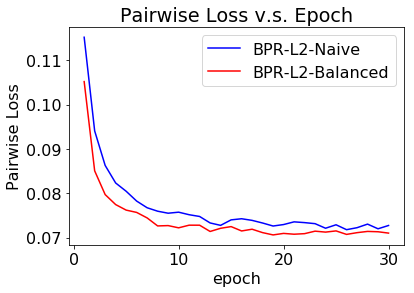
\includegraphics[width=.3\linewidth]{logml-1mpairloss.png}}
\subfloat[Hit Ratio(HR)@10]{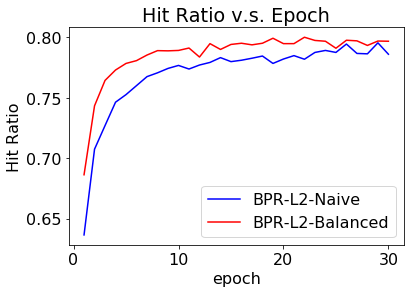
\includegraphics[width=.3\linewidth]{logml-1mhit.png}}
\subfloat[NDCG@10]{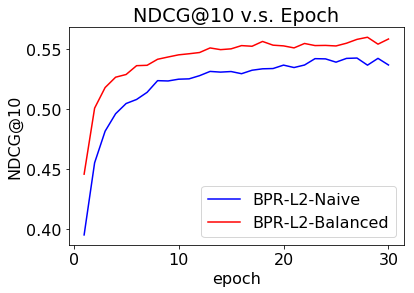
\includegraphics[width=.3\linewidth]{logml-1mndcg.png}}
\caption{MovieLens1m, $r = 100$, $\lambda = 0.1$, stepsize $\eta = 0.1$, compare Naive Sampling and Balanced Sampling with BPR under \textbf{Logistic Loss}}
\label{fig:1m_sample}

\vskip\baselineskip

\subfloat[Pairwise Loss]{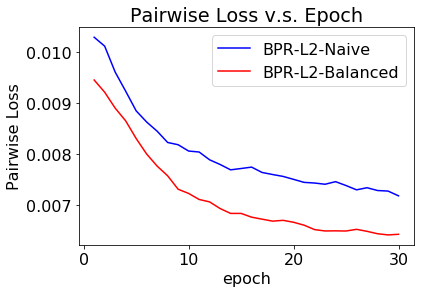
\includegraphics[width=.3\linewidth]{logml-10mpairloss.png}}
\subfloat[Hit Ratio(HR)@10]{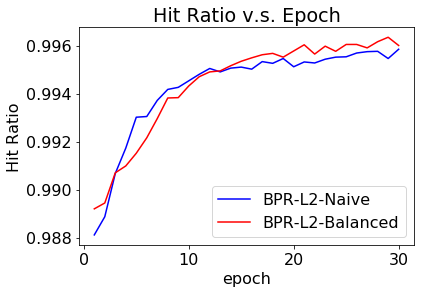
\includegraphics[width=.3\linewidth]{logml-10mhit.png}}
\subfloat[NDCG@10]{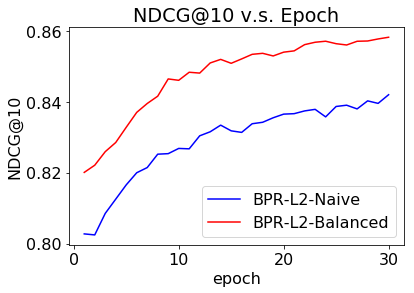
\includegraphics[width=.3\linewidth]{logml-10mndcg.png}}
\caption{MovieLens10m, $r=100$, $\lambda = 0.1$, stepsize $\eta = 0.1$, compare Naive Sampling and Balanced Sampling with BPR under \textbf{Logistic Loss}}
\label{fig:10m_sample}

\end{figure*}

\section{Proof for Theorem 4}

\laks{Theorem 4 can be proved using an argument analogous to that for Theorem 3. Specifically, 
 we need to build an auxiliary function and bound the difference between the empirical risk and the true error. Note that balanced sampling has the same expected true error as the weighted loss used in Theorem 3. Using the same argument as Theorem 3, it is easy to show that balanced sampling and weighted loss share the same property. We omit the details.} 


\section{Supplementary materials for experiments: Comparing Sampling Strategies with BPR under logistic loss}

\laks{The performance of balanced sampling and uniform sampling with BPR under logistic loss is shown in Figures \ref{fig:1m_sample} and \ref{fig:10m_sample}. Our conclusion remains the same, namely that balanced sampling outperforms uniform sampling. Once again, this supports our analytical results.}  






\bibliography{example_paper}
\bibliographystyle{icml2018}


\end{document}


% This document was modified from the file originally made available by
% Pat Langley and Andrea Danyluk for ICML-2K. This version was created
% by Iain Murray in 2018. It was modified from a version from Dan Roy in
% 2017, which was based on a version from Lise Getoor and Tobias
% Scheffer, which was slightly modified from the 2010 version by
% Thorsten Joachims & Johannes Fuernkranz, slightly modified from the
% 2009 version by Kiri Wagstaff and Sam Roweis's 2008 version, which is
% slightly modified from Prasad Tadepalli's 2007 version which is a
% lightly changed version of the previous year's version by Andrew
% Moore, which was in turn edited from those of Kristian Kersting and
% Codrina Lauth. Alex Smola contributed to the algorithmic style files.










